\documentclass[../../thesis.tex]{subfiles}

\begin{document}

\TODO{Introduce the section, what we think and the philosophy of presenting material in such a way.}

\section{Notation}

\begin{itemize}
    \item Encoder $E$
    \item Decoder $D$
    \item Estimated values are presented with a hat, $\widehat{x}$ for a reconstructed value, $\widehat{f}$ for a trained model etc.
    \item Parameters $\theta$ 
    \item Dataset $X = \{x_i\}_{i=1}^N$  
\end{itemize}

\section{Information theoretic/basic stats used in evaluation}

- maximum entropy distribution

- mutual information


\begin{definition}[Differential entropy]
    The differential entropy of a random variable $X$  with pdf or pmf $p$ defined on a sample space $\mathcal{X}$ is
    \begin{equation}
        h(X) =\E[-\log(f(X))] -\sum_{x\in \mathcal{X}} p(x)\log(p(x)),\text{ if $X$ is discrete,}
    \end{equation}
    \begin{equation}
        h(X) =\E[-\log(f(X))] -\int_{\mathcal{X}} p(x)\log(p(x)),\text{ if $X$ is continuous}
    \end{equation}
\end{definition}


- perplexity

\begin{definition}[KL-Divergence]
    For probability distribution $P$ and $Q$ defined on the same sample space $\mathcal{X}$, if for all $x\in\mathcal{X} $ $Q(x)=0$ implies $P(x)=0$, the Kullback-Leibler divergence is defined as
    \begin{equation}
        \KL(P||Q) = \sum_{x\in\mathcal{X}} P(x)\log\left(\frac{P(x)}{Q(x)}\right), \text{ if $P$ and $Q$ are discrete,}
    \end{equation}
    \begin{equation}
        \KL(P||Q) = \int_{x} p(x)\log\left(\frac{p(x)}{q(x)}\right)dx, \text{ if $P$ and $Q$ are continuous}.
    \end{equation}
\end{definition}

\url{https://stats.stackexchange.com/questions/188903/intuition-on-the-kullback-leibler-kl-divergence/189758#189758}

- Cross entropy 

- Graphical probabilistic models 
    - Ancestral sampling

- Generative models


\section{Time Series Inference}
- short-time-fourier transform etc.

\section{Neural Network}
An \textit{artificial neural network} or simply \textit{neural network} is a fundamental model in machine learning, and more specifically in \textit{deep learning}. Neural networks are loosely inspired by the way neurons are assembled in the brain. The model can be traced back the year of 1943 when Warren McCulloch and Walter Pitts developed the first artificial neuron \cite{MCCULLOCH199099}, which is considered to be the first neural model invented. It was first set out in the real world by Frank Rosenblatt in 1957 \cite{rosenblatt1957perceptron}. But not until the development of the backpropagation algorithm in its modern form in the 1980's did the model really gain traction. Neural networks have since then been the highly influential in the development of the machine learning field, with an impressive resume of applications. Some of which, if we stretch the definition a bit, include face recognition, beating humans in chess, Go and Starcraft, self-driving cars and predicting the structure of proteins. The unreasonable effectiveness of neural networks on a broad range of tasks can in part be explained by the \textit{universal approximation theorem}, proven by Kurt Hornlik in 1989 \cite{HORNIK1989359}, which roughly states that a neural network can approximate any (Borel measurable) function to any desired degree of accuracy. 

\begin{figure}
    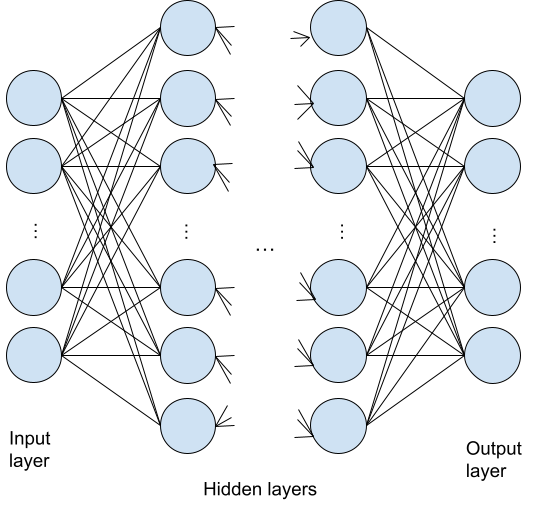
\includegraphics[scale = 0.4]{NeuralNet.png}
    \centering 
    \caption{Illustration of a Neural Network model.}
    \label{fig:NeuralNet}
\end{figure}

A neural network takes in a vector $x \in \mathbb{R}^n$ and builds a nonlinear function $f(x)$ to predict the response $y\in \mathbb{R}^m$. More specifically a neural network maps an input vector $x$ to an output vector $y$ through a series of non-linear functions of linear combinations of the input. This particular structure, presented in figure \ref{fig:NeuralNet} is what distinguishes neural networks from other nonlinear prediction models. The variables $x = [x_1,...,x_n]$ constitutes the units of the \textit{input layer}. The intermediate layers are called the \textit{hidden layers}, and the final mapping to $y$ is called the \textit{output layer}. A neural network is parameterized by a set of \textit{weight} matrices $W_i$ and \textit{bias} vectors $b_i$, together with a specified non-linear \textit{activation function} $\sigma$. We denote the collection of parameters $\{W_1,...,W_{K-1}, b_1,...,b_{K-1}\}$ by $\theta$. Written out a $K$ layered neural network is given by 
\[ 
f_\theta(x) = f_K \circ f_{K-1} \circ \ldots \circ f_2 \circ f_1(x),
\]
where 
$$f_i(x) = \sigma(W_ix+b_i), \quad i \in \{1,...,K-1\},$$ 
and $f_K$ is the output layer, with application dependent structure.\newline
The introduction of nonlinearity by the activation function is what enables the model to approximate nonlinear signals and differentiate itself from a linear regression model. Two of the most commonly used activation functions are $\text{Sigmoid}(x) = \tfrac{1}{1+\exp(-x)}$ and $\text{ReLU}(x) = \max(0,x)$, but countless options exists.\newline
The architecture of neural networks, and most specializations thereof, is sequential in nature. They can effectively be described as compositions of some combination of a flavour of matrix multiplication, non-linear transformation and down or upsampling. 

\subsection{Training Neural Networks}

The training of a neural network is the process of finding values for the weight and bias parameters. The general idea governing neural network training is to optimize the parameters based on some distance metric between the predicted values and the target values. This distance metric is referred to as the \textit{loss function}, and a common choice of loss function is the mean squared error (MSE).\newline

For a multi-variable function $F$ which is differentiable around a point $a$, the direction which it decreases fastest when starting in the point $a$ is given by the negative gradient at $a$, $-\nabla F(a)$. The gradient descent algorithm utilizes this property to find local minima of $F$ by initializing the function with a value $x_0$ and iteratively update 
\[
    x_{n+1} = x_{n} -\gamma \nabla F(x_{n}).
\] 
If the \textit{learning rate} $\gamma$ is small enough we are guaranteed that $F(x_{n+1})\geq F(x_{n})$, and the sequence $x_0,x_1,\dots$ converge to a local minima of $F$.\newline

A neural network $f_\theta(x)$ is itself a multi-variable function, and as long as the loss and activation function are differentiable, the network is as well, both in terms of it argument and parameters. If one differentiates the network with respect to its parameters across its domain, the negative gradient indicates the fastest direction in which to update the parameters to minimize the loss. The optimization problem at hand, for a dataset $X = \{x_i\}_{i=1}^N$ with corresponding labels $Y = \{y_i\}_{i=1}^N$, is
\[
   \widehat{\theta} = \min_{\theta} \frac{1}{N}\sum_{i=1}^N \mathcal{L}(f_\theta(x_i),y_i),
\]
and one would iteratively update the parameters by gradient descent 
\[
    \theta_{n+1} = \theta_{n} - \frac{\gamma}{N}\sum_{i=1}^N\nabla_\theta \mathcal{L}(f_\theta(x_i),y_i).
\]

If the dataset $X$ is large, the gradient calculations are expensive. In these cases, which in modern machine learning is the standard scenario, an effect estimator for the true gradient is used instead. Stochastic gradient descent (SDG) is a very popular approach. Instead of computing the gradient at each datapoint every iteration, SDG updates the parameters by iterating through the dataset and using the gradient at each single datapoint. The dataset is then permuted and iterated through again until an approximate minimum is reached. Pseudocode of SDG is presented in algorithm \ref{alg:SDG}.

\begin{algorithm}
\caption{Stochastic Gradient Descent (SDG)}
\label{alg:SDG}
\begin{algorithmic}
    \State Initialize parameters $\theta$ and learning rate $\gamma$
    \While{Not converged} 
        \State Permute training set $(X,Y)$
    \For{$i$ in $1,\dots,N$}
        \State $\theta \gets \theta - \gamma\nabla_\theta \mathcal{L}(f_\theta(x_i),y_i)$
    \EndFor
    \EndWhile
\end{algorithmic}
\end{algorithm}
\TODO{Mini batch SDG}

For the actual gradient computations, the backpropagation algorithm is used. It provides an efficient way of computing gradients in neural networks by leveraging the compositional structure. In essence backpropagation is an efficient application of the Leibniz chain rule for differentiation.\newline

For a through introduction to the subject of neural networks and the training thereof we refer to chapter 6 and 8 of \cite{deeplearningbook}.


\section{Convolutional Neural Network}
This section draw inspiration on the presentation of convolutional networks in chapter 9 of \cite{deeplearningbook}.\newline

A convolutional neural network (CNN) is a particular type of neural network that is developed to learn local features in the data. This local feature learning is enabled by the mathematical operation of convolution. In essence a CNN is a neural network where matrix multiplication is switched for convolution at least one of the layers \cite{deeplearningbook}. \newline
Fully connected neural networks have a fundamental drawback in that their computational complexity grows intractably large when the input dimensionality is high. This makes them unsuited for high dimensional data, such as images. Convolutional neural networks directly address this issue via various downsampling techniques. Convolutional neural networks has a rich history and a long track record of success stories. They are inspired by the architecture of visual cortex cells in mammals. Inspired by the discovery of Hubel and Wiesel \cite{https://doi.org/10.1113/jphysiol.1968.sp008455} the neocognitron was proposed in 1980\cite{6313076}. The neocognitron is widely considered the predecessor of convolutional neural networks. In 1989 Yann LeCun et al. introduced the modern framework for CNNs \cite{LeCun1989ConvNet} and demonstrated its effectiveness on the task of hand written digit recognition. Since then CNNs have been an indispensable part of machine learning research, especially in the computer vision domain. For an exposition on the advances on convolutional neural networks and its applications we refer to \cite{gu2017recent}.

\subsection{The convolution operation}

% "Convolution leverages three important ideas that can help improve ML systems: sparse interactions, parameter sharing and equivariant representations" \cite{deeplearningbook}.

The convolution operation is an integral transform with extensive applications. It generalizes the notion of a moving weighted average. In mathematics it is ubiquitous because of its relationship with the Fourier transform.\newline

Let $f$ and $g$ be real valued functions, then their convolution is defined as
\begin{equation}
    (f*g)(t) = \int_{-\infty}^{\infty} f(\tau)g(t-\tau) d\tau
\end{equation}

The mathematical nuances of the exact criteria for the above integral to exist is outside the scope of this thesis, and not particularly relevant. But if $f$ and $g$ are integrable (in the Riemann or Lebesgue sense) then the convolution exists. As a rule of thumb, the convolution of $f$ and $g$ is as "smooth" as the smoothest of $f$ and $g$. It is worth mentioning that convolution is commutative, i.e that $f*g = g*f$, which can be seen by a simple change of variables. \newline

As is typical for integral transforms, the function $g$ is referred to as the \textit{kernel}. In the context of convolutional networks the kernel consists of learnable parameters and the function $f$ is the \textit{input}. The output is referred to as the \textit{feature map} \cite{deeplearningbook}. In machine learning we handle discrete signals, represented as multidimensional arrays. As a result we must employ a discrete variation of the convolution operation. Let $I$ be the input and $K$ be the kernel, both discrete, then their convolution is defined as
\begin{equation}
    (I*K)[n] = \sum_{m=-\infty}^{\infty} I[m]K[n-m].
\end{equation}
In practice $I$ and $K$ typically has finite support, i.e they are zero for large positive and negative arguments, which circumvents any convergence problem.\newline
Convolutions are naturally defined for higher dimensional functions by component wise extension. For a two dimensional image $I$ and a kernel $K$ we calculate their convolution as 
\begin{equation}
    (I*K)[i,j] = \sum_{n=-\infty}^{\infty}\sum_{m=-\infty}^{\infty} I[n,m]K[i - n,j - m]. 
\end{equation}
The operation is illustrated in figure \ref{fig:Convolution}.
\begin{figure}[h]
    \label{fig:Convolution}
    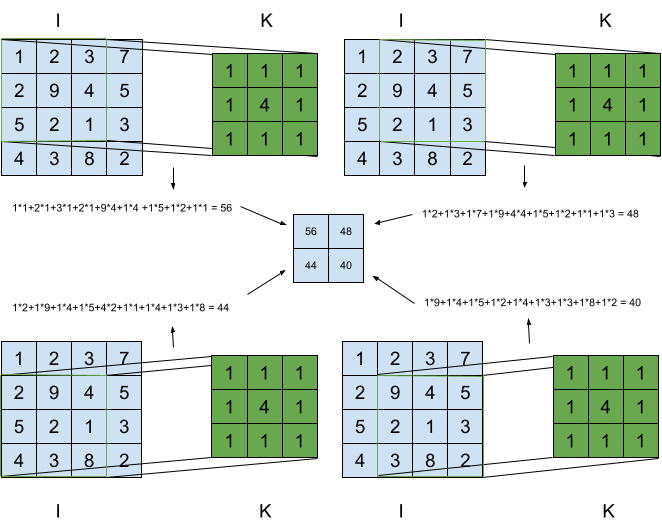
\includegraphics[scale=0.5]{Convolution.png}
    \centering    
    \caption{Illustration of discrete two dimensional convolution}
\end{figure}

Convolution in machine learning does not always correspond exactly to the mathematical definition of the operation, but rather to cross-correlation. The difference is just a sign flip in the kernel arguments. Operation is no longer commutative, but in practice this does not affect anything as the learned kernel parameters will be equivalent \cite{deeplearningbook}.\newline
%  Machine learning applications are focused on what works, rather than writing proofs. 

In the field of digital signal processing discrete convolutions are used extensively. Traditionally predefined kernels are used to alter a signal in predictable ways. Two well known kernels are Gaussian and edge detection kernels. Gaussian kernels are two dimensional gaussian distributions and are used for blurring. Edge detection kernels are designed in such a way that areas of similar intensity are mapped to $0$ and areas of variable intensity are mapped to high values. In figure \ref{fig:kernelIllustration} we demonstrate the effect of two such kernels. Edge detection in particular provide a hint to how CNNs learn interesting features in the data. In a convolutional layer the kernels are learned such that the feature map is helpful for the training objective. 
\begin{figure}[h]
    \centering
    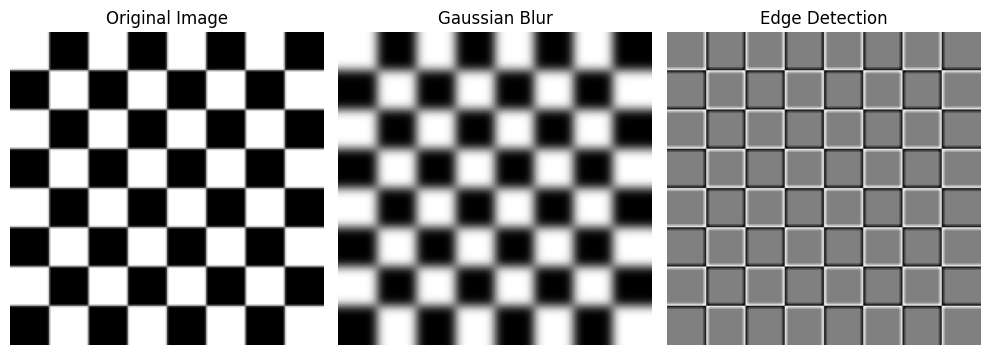
\includegraphics[scale = 0.5]{Kernel_illustration.png}
    \caption{Illustration of discrete convolution applied to images. Image part of Scikit-image data package.}
    \label{fig:kernelIllustration}
\end{figure}

\subsection{Pooling}
As mentioned earlier CNNs are mainly used when the data has high dimensionality. In order to reduce the dimension to a manageable level \textit{pooling} is used. A pooling operation is applied as a down sample technique on feature maps, replacing regions of the output with summary statistics. Two of the most common are max and average pooling, which replaces the region by its maximal or average value respectively. There are two hyperparameters for any pooling operation, the filter size, which determines the region of values to calculate the summary statistic, and stride length, which determines how the filter moves across the feature map. In addition to dimension reduction, pooling assist in making the representations approximately invariant to small distortions of input. Illustrations of max pooling with different stride is presented in figure \ref{fig:mp2} and \ref{fig:mp2}, while the effect of max and average pooling on image data is illustrated in \ref{fig:mean_max_pool}.

\begin{figure}[h]
    \label{fig:mp2}
    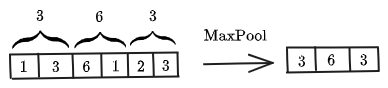
\includegraphics[scale=0.5]{MP_stride2}
    \centering    
    \caption{Max pooling of one dimensional array. Filter size: $2$, stride: $2$.}
\end{figure}
\begin{figure}[h]
    \label{fig:mp1}
    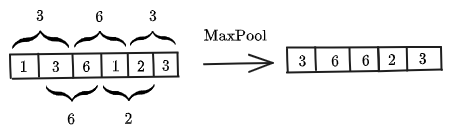
\includegraphics[scale=0.5]{MP_stride1}
    \centering    
    \caption{Max pooling of one dimensional array. Filter size: $2$, stride: $1$.}
\end{figure}

\begin{figure}[h]
    \label{fig:mean_max_pool}
    \centering
    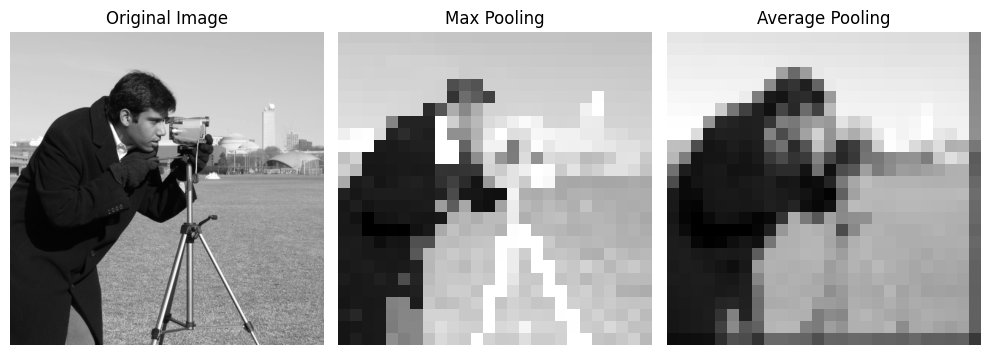
\includegraphics[scale = 0.5]{pooling_illustration.png}
    \caption{Illustration of mean and average pooling applied to images. Filter size and stride is $20\times 20$. Original image size is $512\times 512$, pooled images are $26\times26$. Image part of Scikit-image data package.}
\end{figure}


\subsection{Architecture}
There is a large variety of specific architectures which fall in the category of a CNN, but their basic components are largely the same. They consist of convolutional layers, pooling layers and fully connected layers. In figure \ref{fig:LeNet5} an illustation of the original LeNet-5 \cite{LeCun1989ConvNet} is presented as an illustration of a general CNN.\newline

\textbf{A convolutional layer} consists of several kernels used to compute different \textit{feature maps}. Each kernel convolved with entire input, and the different feature maps are produced by changing kernel. A nonlinear activation function is then applied pointwise to the feature maps.
\begin{figure}[h]
    \centering
    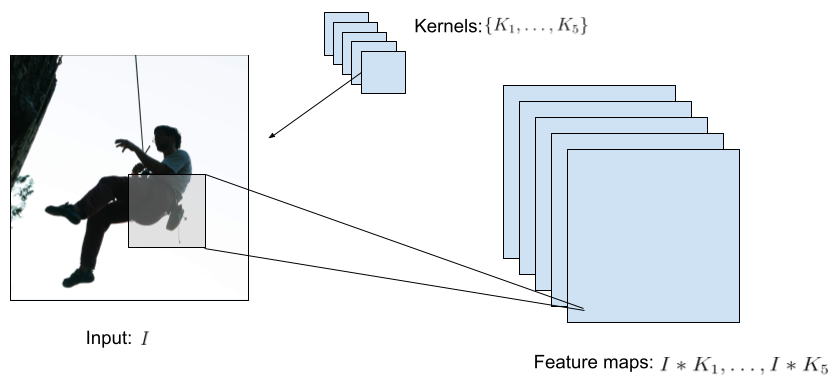
\includegraphics[scale = 0.5]{convlayer.png}
    \caption{Convolutional layer.}
\end{figure}
\textbf{A pooling layer} is typically placed between convolutional layers and work as a stronger downsampler which aims to enforce approximate translation invariance. A pooling operation is applied across each feature map.\newline

\textbf{The fully connected layer} is just your typical hidden layer in a neural network, i.e connect every input to every node in the output. Because of computational issues mentioned earlier fully connected layers are first introduced when the input data has been sufficiently downsampled.

\begin{figure}[h]
    \centering
    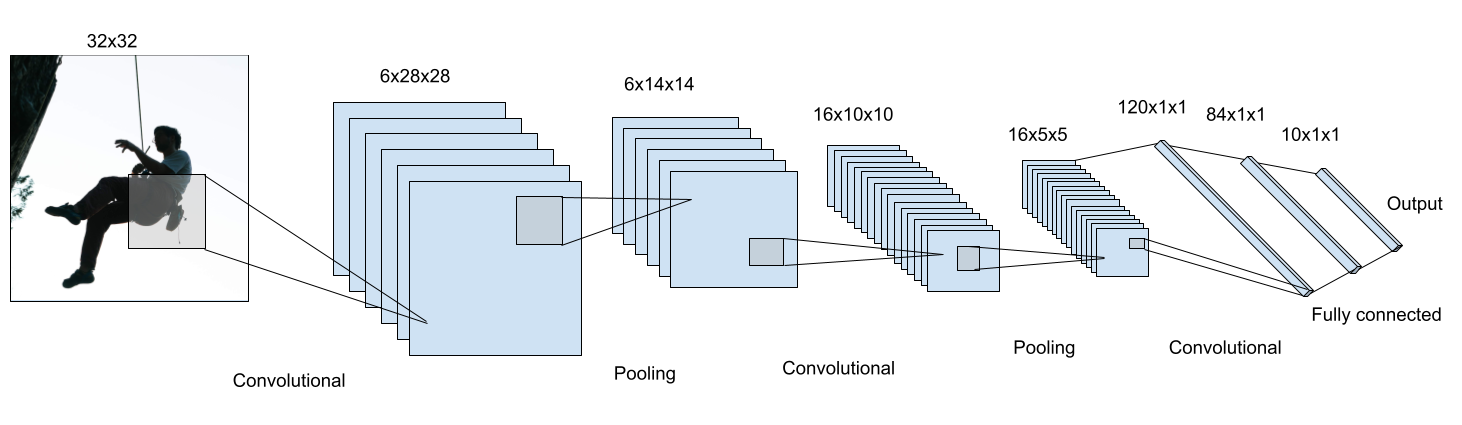
\includegraphics[scale = 0.25]{LeNet5.png}
    \caption{LeNet-5 network \cite{LeCun1989ConvNet}}
    \label{fig:LeNet5}
\end{figure}


\subsection{Transposed Convolutional Networks}
Transposed convolution or deconvolution, also known as fractionally-strided convolution is a technique used to reverse the downsampling from convolutions. In essence it is an inpainting or upsampling technique known from digital signal processing. The flexibility of learning data dependent transposed convolutional kernels enables one to more effectively reverse the downsampling from convolutional layers. They are extensively used in combination with convolutional downsampling in \textit{encoder-decoder architectures} presented in section \ref{section:VQVAE}.  

\begin{figure}[h]
    \centering
    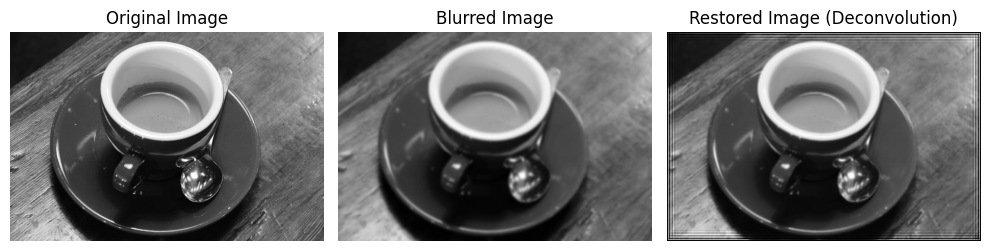
\includegraphics[scale = 0.5]{deconv_illustration.png}
    \caption{Illustration of deconvolution applied to images. Here using Gaussian blur and restoring using the Richardson Lucy algorithm with a Gaussian deconvolution kernel. Image part of Scikit-image data package.}
\end{figure}


% \section{Residual Neural Network}

% Deep neural networks are hard to train. But we want deeper networks as the representations learned in deeper networks tend to be higher level/more abstract \cite{zeiler2013visualizing}. 

% The problem of exploding/vanishing gradients \todo{write about and explain what this is} has been to a large extent been solved by normalized initialization and intermediate normalization layers. This has enabled networks of tens of layers to start converging for SDG with backprop \cite{he2015deep}. \TODO{Rewrite the above in more of my own words}.



% The degeneration problem: 

% The deep residual learning framework was developed to address the degeneration problem.

% \cite{he2015deep}

% \section{Dimension reduction/visualization techniques}

% \subsection{PCA}
% Principle component analysis i a linear dimmension reduction technique which provides the axes of a point cloud 
%  PCA provides a linear projection on the eigenspace of the covariance matrix of the data. 



% \subsection{t-SNE}
% \cite{t-SNE}
% T distributed stochastic neighnourhood encoding.

% \subsection{UMAP}
% \cite{mcinnes2020umap}

% \subsubsection{densMAP}


\section{Representation Learning}

The focus of this thesis is representation learning for improved time series generation.

\subsection{What a representation?}

Representation learning is a term not too easily defined, one reason being the abstraction level. It is helpful to first consider what is meant by \textit{representation} of information. Lets begin by walking through a familiar and illustrative example. Consider the base ten integer $(4)_{10} = 4$. The number can equivalently (in terms of information content) be expressed, that is represented, in any other base. The particular base we choose depends on our intention with the number. If we want to work with digital electronics, a binary representation ($(4)_{2} = 10$) is very useful, as transistors has two states. When humans do arithmetic, base ten representations of the integers are very natural, as we have ten fingers. A particular representation of information can make a task easier or harder. The information content is unchanged by a change of representation. What is changed is the easiness or difficulty of certain information processing tasks. Representation learning is then the process of learning a certain representation of information. \newline
Representations are too highly dependent on who, or what, that will process it. An example is time. Humans have developed a standardized system for writing timestamps which works fairly well for us. But, if we want to model time dependent phenomena, say using tabular data, the DateTime representation is of very little help to a tree based model for instance. The reason being that the numerical representation of timestamps close in time is not necessarily close in numerical value. Think of 23:59 to 00:00. A possible solution is to change the representation such that the numerical values actually respect the periodic nature by mapping to the circle. The new representation is then useless for humans, but quite a lot more useful to a computer. Representation learning in machine learning can thus be thought of as algorithms which are designed to learn representations which is useful for a ML objective.

\subsection{Why do we care about representation learning?}
Those who has worked with data science or machine learning and has come across feature engineering are familiar the effect good feature engineering has on a models performance. The same people too knows the level of domain expertise, creativity and time is needed to feature engineer well. In reality much of the actual time spent in the process of deploying machine learning methods revolves around constructing good data pipelines and applying transformations that produce representations beneficial for the algorithm at hand \cite{Rep-rev-persp}. Thus the ability to automate such tasks would be incredibly beneficial, and ease the use of ML algorithms significantly. It is here one of the intriguing and promising features of neural networks, with its many specializations and architectures, comes into play. They have shown the ability to learn useful abstract representations of the data and provide automatic feature engineering \cite{Rep-rev-persp}. 


\subsection{What is a good representation?}

The goodness of a representation is then determined by how easy it makes a subsequent task. The concept of universally good representations is ill-defined, for any representation extracted of a non-invertible function, a \textit{downstream tasks} can be designed (in principle) to based on the lost information, hence achieve arbitrarily bad performance. There is no free lunch in representation learning either. One must specify a set of predefined downstream tasks, and evaluate according to those. Intuitively the quality of the representations are also considered higher if the the representations is able to perform well on several downstream tasks i.e when they are more general. 

\subsection{How does one evaluate representations?}
There are several different evaluation protocols in representation learning. They involve training a model on a \textit{pretext task}, which as defined in \cite{jing2019selfsupervised} is a task for a network to solve, where the goal is to learn representation. Then the learned representations are evaluated on a downstream task. In general the downstream task is solved in a supervised manner, using human annotated data.\newline

In a $N$-layered network $f = f_N\circ ...\circ f_1$, the intermediate value of the data $x$ in some layer $n$ is what is meant by the networks learned feature representations. When we are interested in the representations learned it thus is helpful to dissect a model $f$, notation wise, into a \textit{feature extractor} $h$ and an \textit{output function} $g$ such that it can be factored as $f = g \circ h$. Representation learning algorithms typically follow the pattern
\begin{itemize}
    \item Train $f= g \circ h$ on a pretext task.
    \item Discard $g$
    \item Use the learned feature extractor $\widehat{h}$ as part of a new model.
    \item Evaluate the new model on the downstream task. 
\end{itemize}



The standard evaluation protocol is to train a linear head $g_D$ on top of the \textit{frozen} representations in a supervised manner and evaluate this models performance. This is to say that we train  $f_D = g_D\circ \widehat{h}$ by only updating the parameters of the linear model $g_D$, and evaluate $\widehat{f}_D$ on some test set. This protocol is sometimes referred to as \textit{linear probing}. A common downstream task is classification, where the idea is that good and informative representations should differentiate data in such a way that it is easy to separate them. \newline

An common alternative protocol is similar to the one above, but rather than freezing the feature extractor one let all parameters of $f_D$ to be learnable on the downstream task. This protocol is referred to as a pretraining-finetuning. \newline

It is of interest how $f_D$ performs in terms of accuracy on the downstream task and training time, and too how these sensitive metrics are to training data size. The baseline comparison would then be an identical but randomly initialized model. It is considered highly advantageous if one is able to pretrain a feature extractor using cheap and abundant data in a way which ensures faster convergence on a downstream task where data is expensive or scarce.\newline

It is with mentioning that in cases where the sole goal is to create the best performing model, a more complex task specific head $g_D$ is often used. For a comprehensive survey on representation learning we refer the reader to \cite{nozawa2022empirical}.


\begin{figure}[h]
    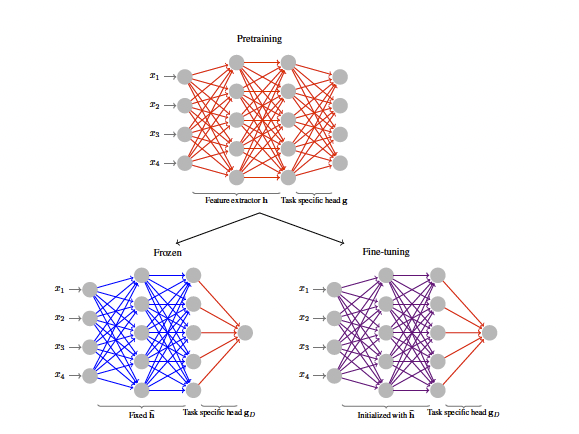
\includegraphics[scale=0.5]{rep_learnin_protocol.png}
    \centering    
    \caption{Taken from \cite{nozawa2022empirical}}
\end{figure}


\section{Transformers}

Since their introduction in the seminal paper titled "Attention is all you need"\cite{vaswani2023attention} transformers have taken the field of machine learning and artificial intelligence by storm. It is the enabling architecture behind large language models (LLMs) such as Googles BERT, Metas Llama and OpenAIs ChatGPT. Drawing inspiration from the initial success in natural language processing vision transformers \cite{dosovitskiy2021image} were developed for computer vision applications, and similar trends are shown for other modalities such as audio \cite{latif2023transformers} and time series \cite{wen2023transformers}. \newline
Transformers were developed for sequential modelling and has capabilities of learning far ranging dependencies in data through the \textit{multi-headed attention mechanism}. In the realm of sequential modelling recurrent neural networks \todo{cite} and long short-term memory neural networks\todo{cite} were the previous state of the art, but modeling long term dependencies has proven difficult \cite{279181} as one encounters the \textit{vanishing or exploding gradient problem}. One of the main novelties of the transformer architecture is not relying on recurrence, and instead solely using the attention mechanism to capture dependencies between input and output.
\newline
The transformer takes as input a sequence of symbols. This means in particular that for a specified modality, e.g text, speech, image and time series, they must first be translated into a sequence of symbols. This is accomplished by a process called \textit{tokenization}. The conceptually easiest word-level tokenization in NLP, where one creates a dictionary of all words in the dataset, and assigns to them an integer value. A piece of text can then with relative ease be mapped to a sequence of integers. Other modalities as speech, image and time series are usually represented as matrices and can therefore naively be modeled as a sequence numbers. Because of the high dimensionality, this would require a significant amount of computational resources. In addition the transformer would need to model incredibly far ranging dependencies and handle redundant information. Hence various tokenization methods are used to represent the data as coarser sequences. 
\newline
Transformers can be adopted for generative tasks, and has done so with great success. Autoregressive transformers such as the GPT series are trained to predict the next token in a sequence given the preceding tokens. By treating images as sequences of patches vision transformers can generate new images or inpaint missing patches conditional on the input. With the introduction if vision transformers \cite{dosovitskiy2021image}, input images were split into patches and linearly projected before being processed by the transformer. Since then \textit{Vector-Quantized}-based tokenization introduced by \cite{VQVAE} has emerged as a popular approach.

\subsection{The attention mechanism}

\begin{figure}[h]
    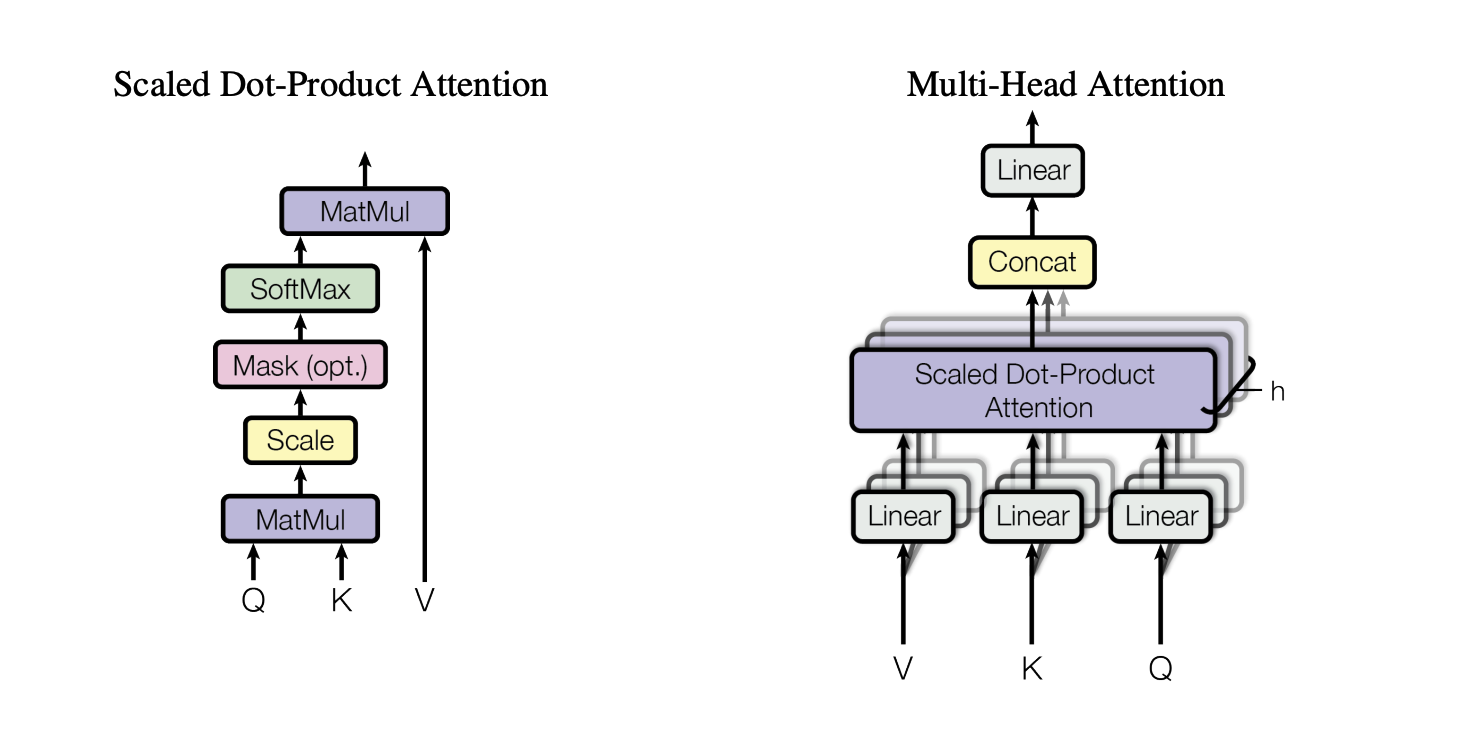
\includegraphics[scale=0.25]{Attention.png}
    \centering 
    \label{fig:attention}
    \caption{(left) Scaled dot-product attention. (right) Multi-headed attention. Taken with permission from \cite{vaswani2023attention}}
\end{figure}

"Attention can be described as mapping a query and a set of key-value pairs to an output, where the query, keys, values and outputs are all vectors". Scaled dot-product attention is computed by 

\begin{equation}
    \text{Attention}(Q,K,V) = \softmax \left(\frac{QK^T}{\sqrt{d_k}}\right)V
\end{equation}

Multi-headed attention projects the inputs $Q,K,V$ down to $h$ subspaces, where the scaled dot product attention is applied to each subspace. The individual attention heads are concatenated before passing through a final linear layer. That is to say 

\begin{equation}
    \text{MultiHead}(Q,K,V) = \text{Concat}(\text{head}_1,\dots, \text{head}_h)W^O,
\end{equation}
where
\begin{equation}
    \text{head}_i = \text{Attention}(QW_i^Q,KW_i^K,VW_i^V). 
\end{equation}

The multi-headed attention enables the transformer to focus on different aspects of the input sequence simultaneously. 

\subsection{Architecture}


\begin{figure}[h]
    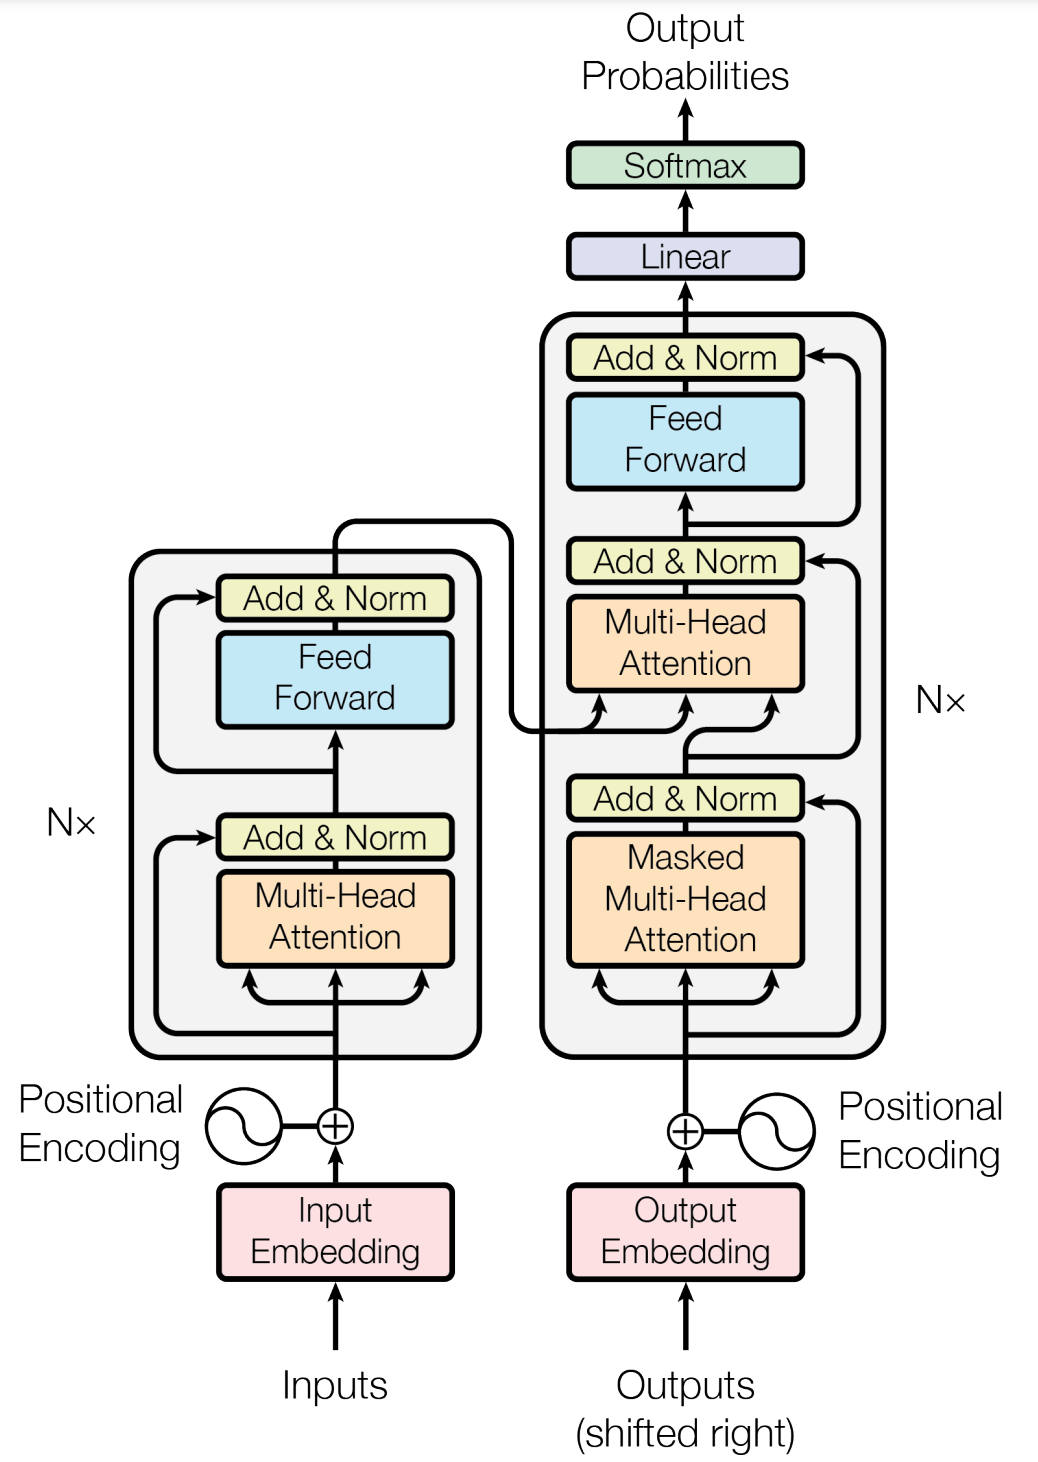
\includegraphics[scale=0.1]{Transformer_architecture}
    \centering 
    \label{fig:transformer}
    \caption{The Transformer - model architecture. Encoder (left), decoder (right). Taken with permission from \cite{vaswani2023attention}}
\end{figure}
An overview of the original transformer architecture is presented in figure \ref{fig:transformer}. The architecture has several distinct components.
\newline

\textbf{Embeddings}: The input embedding maps each token in an input sequence to a vector. The input embedding is essentially a lookup table. 
\newline

\textbf{Positional encoding}: The transformer does not rely on convolution or recurrence to make use of the order of the input sequence. Instead it relies on a positional encoding, which is done by adding information about the relative position of an element in the embedded sequence. In the original paper \cite{vaswani2023attention} sinusoids are used to encode the position with unique values. 
\newline

\textbf{Encoder}: The embeddings with positional encodings are passed through the transformer encoder, which consist of $N$ identical layers. The layers consist of the multi-head attention and a fully connected neural network, with residual connections and normalization at each sublayer. 
\newline

\textbf{Decoder}: The decoder similarly consists of $N$ identical layers. They consist of a masked attention layer, which prevents the decoder to utilize future values in the sequence during training, a multi-head attention applied to the output of the encoder and a fully connected neural network. All sublayers employ residual connections and normalization. The output is converted to probabilities in the standard way by a linear layer followed by softmax. 
\newline

Bidirectional transformer models such as BERT \cite{devlin2019bert} use an encoder only architecture, which enables the attention to attend both directions. The issue of "seeing in the future" is resolved by a training technique referred to as \textit{Masked modelling} \ref{section:Masked modelling}.

\section{Self-Supervised learning}

Self-supervised learning (SSL) has had great success in natural language processing and computer vision in recent years, and is quickly being applied for other modalities. In our work we leverage SSL for representation learning in the time series domain. Before we introduce SSL, it is with mentioning that machine learning models can be coarsely divided into two categories of learning, supervised and unsupervised. 
\newline
Supervised learning refers to models who learn using labeled data. That is to say for a given input $x$ we already know what the desired output $y$ is during training, and can therefore supervise (update) our models parameters by directly comparing model output and the true value. A bit more formally, for a dataset $X = \{x_i\}_{i=1}^N$ with corresponding human annotated labels $Y = \{y_i\}_{i=1}^N$, the objective of a supervised learning algorithm is to fit $f_\theta$ in such a way that the loss across the data is minimized
\begin{equation}
    \widehat{f}_\theta = \min_\theta \frac{1}{N} \sum_{i=1}^N L(f_\theta(x_i),y_i).
\end{equation}
Common approaches to supervised learning for neural networks is to calculate some distance metric between the predicted value $\widehat{y}$ and the true value $y$ and update parameters by backpropagation.\\\\
The models falling under the supervised learning category are widely deployed and has seen tremendous success. Classical statistical models, as well as support vector machines and decision tree based models are all examples of models in this learning paradigm. The main issue with supervised learning is the need for labeled data, and labeled data is in many ways scarce.
\newline

Unsupervised learning on the other hand refers to models or algorithms who learn exclusively from unlabeled data. That is to say that the models learn intrinsic patterns in the data. Examples of unsupervised learning models are clustering methods as K-means, K Nearest Neighbor and Gaussian mixture models, dimension reduction techniques as PCA and SVD and neural network architectures such as Autoencoders. Unsupervised algorithms are used extensively in exploratory data analysis, data visualization and clustering. In a world with abundant unlabeled data, good unsupervised techniques are quite valuable. Until recently such techniques have been hard to come by and typically fallen short compared to supervised approaches. 
\newline

Self-supervised learning is subcategory of unsupervised learning which has shown great success within NLP and computer vision, closing in on the state of the art supervised representation learning \cite{bardes2022vicreg} \cite{zbontar2021barlow}. SSL refers to model who use the data itself to generate a supervisory signal, rather than external labels as in supervised learning. Even as SSL is considered unsupervised learning, the learning formulation is quite similar to that of supervised learning.\newline

For a dataset $X = \{x_i\}_{i=1}^N$ with \textit{pseudo labels} $P = \{p_i\}_{i=1}^N$ the objective of a self-supervised learning algorithm is to fit $f_\theta$ in such a way that the loss across the data is minimized. In other words find 
\begin{equation}
    \widehat{f}_\theta = \min_\theta \frac{1}{N} \sum_{i=1}^N L(f_\theta(x_i),p_i).
\end{equation}

A pseudo label is an automatically generated label from the data. In \textit{siamese} architectures the pseudo labels are typically some \textit{augmentation} of the original data.\newline

SSL has in recent times been a fruitful approach to unsupervised representation learning and has played an integral part in the boom of large language models together with the invention of the transformer architecture. With models growing ever larger and more data hungry, SSL is essential in pretraining. Randomly initialized networks are difficult to train and requires a lot of time and computational resources. SSL has shown remarkable results when used for pretraining. That is as models for learning network parameters who capture semantics of data, without the need for labels. Pretraining networks enables foundation models, which can be trained for many different tasks in a supervised fashion requiring a lot less resources.\newline

Many successful SSL models in the computer vision domain share a similar architecture.

\subsection{Siamese Architecture-based SSL }
A siamese network architecture \cite{siamese} consists of two networks, called branches, with a shared encoder on each branch. Such networks are trained to produce similar representations for different views of the same data. In models with such architecture, the existence of trivial solutions, such as both networks ignoring input and produce identical constant embeddings, is a major issue. This issue is referred to as \textit{collapse} of the model.\newline

In the computer vision domain several representation learning algorithms utilizing a siamese architecture have been proposed. They mainly fall under two categories: \textit{contrastive} and \textit{non-contrastive} SSL.\newline

Contrastive SSL uses positive and negative samples and learns representations by pulling positive pairs closer together and negative pairs further apart. Examples include MoCo \cite{he2020momentum} and SimCLR \cite{chen2020simple}. SimCLR constructs two correlated samples by applying augmentations to an input sample, and considers these as positive pairs. Contrastive methods requires large batch sizes as well as a large number of negative pairs compared to positive in order to learn representations effectively \cite{lee2024computer}. These obstacles lead researchers to look elsewhere.\newline

Non-Contrastive SSL methods such as BYOL \cite{grill2020bootstrap}, BarlowTwins \cite{zbontar2021barlow} and VIbCReg \cite{computer} circumvent the need for positive and negative pairs while simultaneously avoiding model collapse by different methods. Common for all is the use of augmentations, a transformation of the input that works as a pseudolabel. The models learn to map representations of the input and augmentation closer together. In order to avoid collapse BYOL introduces asymmetry in the architecture as well as the stopgradient operation, Barlow Twins minimizes the information redundancy between the two branches and VIbCReg by maintaining the variability in each branch while decorrelating features. Common for all is the ability to learn useful representations.

% \cite{mialon2024variance} VCReg for pairwise independence in SSL representations. 

\subsection{Masked modelling}
\label{section:Masked modelling}
Masked modelling is a conceptually simple self-supervised learning technique for generative models. The idea is to mask or cover a portion of the data and predict the masked portions. By comparing the prediction against unmasked data the model can learn useful representations without supervision. Since the introduction of masked modelling in natural language processing by \cite{devlin2019bert} it has been the de-facto standard for self-supervised pretraining of language models. BERT introduced masked modeling for language representation learning as means to use bi-directional transformers without enabling each word to "see itself". \newline
% \TODO{When did GPT \cite{Radford2018ImprovingLU} use Masked modelling?}

In the computer vision domain masked modelling has too gotten much attention. Early works in masked image modelling \cite{he2021masked} attempted to mask image patched directly with some success. But when vision transformers \cite{dosovitskiy2021image} surpassed CNN in 2021\cite{he2015deep}, CV research began to draw inspiration more heavily from \cite{devlin2019bert} and began tokenizing images and pretraining transformers. In 2022 MaskGIT\cite{chang2022maskgit} proposed masked visual token modelling , utilizing vector-quantized-based tokenization together with a bidirectional transformer. For a thorough survey on masked modelling for SSL in the vision domain we refer to \cite{li2024masked}. 

\section{Vector Quantized Variational Autoencoder (VQVAE)}
\label{section:VQVAE}
Our model is based on the Vector Quantized Variational Autoencoder (VQVAE) introduced in \cite{VQVAE}, and includes an Auto-encoder (AE) branch. Therefore it is natural to dive into the models. We first start with introducing auto-encoders, then present the variational variation VAE before presenting VQVAE. 

\subsection{Autoencoder (AE)}

Consists of two neural networks, an encoder $E$ and decoder $D$. They can be seen as maps between spaces $X$ and $Z$, where we refer to $X$ as the data space and $Z$ as the latent space. 
\begin{equation}
    X \xrightarrow{E} Z \xrightarrow{D} X 
\end{equation}

\begin{figure}[h]
    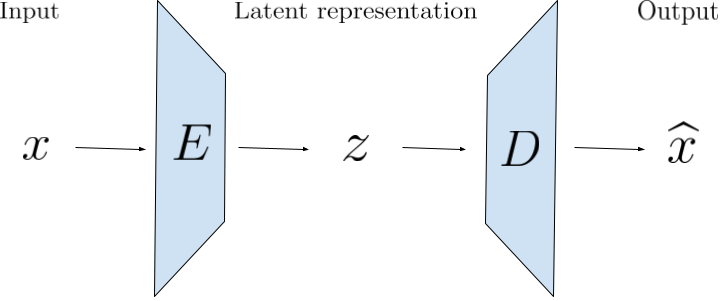
\includegraphics[scale = 0.3]{Autoencoder.png}
    \centering
    \caption{Schematics of the autoencoder architecture.}
    \label{fig:autoencoder}
\end{figure}

The autoencoder is trained in such a way that the composition of encoder and decoder is approximate to the identity. Typically the dimension of the latent space is much lower that that of the data space. Encoder and decoder then compresses and decompresses the data and learns efficient \textit{latent representations}. 
\TODO{Information bottleneck}
\TODO{Issues with latent representations and the need for regularization}

\subsection{Variational Autoencoder (VAE)}
Variational Autoencoders (VAE) were introduced in \cite{kingma2022autoencoding} and is a variational Bayes approach to approximate inference and learning with directed probabilistic models. The architecture of VAE is similar to AE, but the mathematical formulation is quite different. For context variational inference is a technique in statistics used to approximate complex distributions by looking for the closest approximation within a simple, but flexible, parametric family. \newline 

In the VAE framework we assume that the dataset $X = \{x_i\}_{i=1}^{N}$ consists of iid samples from a random variable $\mathbf{x}$. We further assume that the data is generated by some unobservable random process. This is to say that we assume there is a random variable $\mathbf{z}$ such that $x_i \sim p_{\theta^*}(x|z_i)$, where $z_i \sim p_{\theta^*}(z)$. The distribution $p_{\theta^*}(z)$ is referred to at the true prior and $p_{\theta^*}(x|z_i)$ as the true likelihood. As $\mathbf{z}$ is unobservable and the true distributions are unknown, one has to assume their form. In general the prior and likelihood are assumed to be from parametric families $p_{\theta}(z)$ and $p_{\theta}(x|z)$. As with any model where one wishes to employ gradient based learning, the distributions are assumed to be differentiable almost everywhere, both with respect to their parameters and argument.\newline
\begin{figure}[h]
    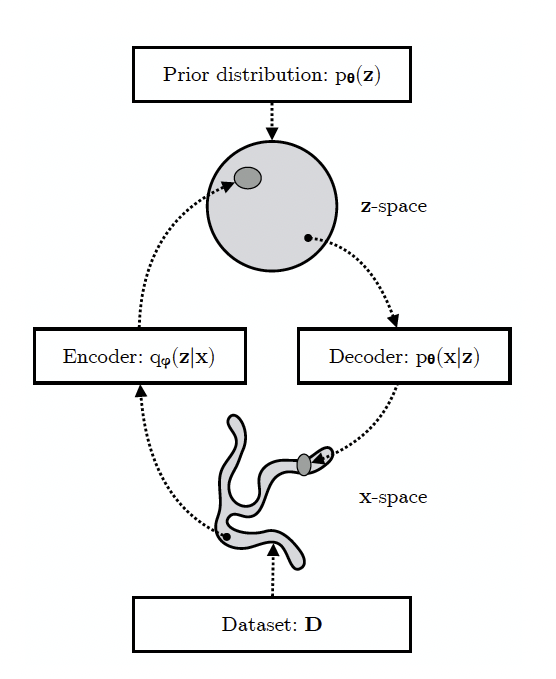
\includegraphics[scale=0.3]{VAE}
    \centering  
    \caption{\cite{VAE}, need to ask for permission or make own}  
\end{figure}

VAEs have two components to their architecture. The first is a probabilistic encoder, often called the inference model, $q_\phi(z|x)$ which approximates the true posterior. Secondly a probabilistic decoder, often called the generative model $p_\theta(x|z)$, which approximates the likelihood. These models are typically parameterized by some type of neural network, and in that case $\phi$ and $\theta$ are the weights and biases of the two networks. Given a datapoint $x_i$ the probabilistic encoder provides a distribution over the possible values of the latent variable $\mathbf{z}$. Similarly, given a latent representation $z_i$ the probabilistic decoder produces a distribution over the possible corresponding values of $\mathbf{x}$. \newline

The probabilistic part of the encoder and decoder is the sampling. The output for a given $x$ or $z$ is a distribution, and for the same input the same output distribution is calculated (as long as the network parameters are frozen). Actually $x$ and $z$ are mapped to the parameters of a distribution, which uniquely determines the distribution in a particular family.\newline

The most common situation is to assume 
\begin{itemize}
    \item Prior $p_\theta(z)\sim N(0,I)$
    \item Likelihood $p_\theta(x|z)\sim N(D(z), I)$
    \item Variational posterior $q_\phi(z|x)\sim N(E(x)) = N(\mu_x, \Sigma_x)$
\end{itemize}
The encoder maps datapoints to parameters of the variational distribution, i.e the approximate posterior $q_\phi$, $x \mapsto E(x) = (\mu_x, \Sigma_x)$. A latent representation $z$ is then sampled from $q_\phi$, which constitutes the random part of the algorithm. The decoder maps $z$ to the expected value of the likelihood $p(x|z)$, $z_i \mapsto D(z_i)$. \newline

There are several reasons for choosing Gaussian distributions, one being that the Gaussian distribution a scale-location family. This enables us to circumvent the problematic random component in the VAE when using gradient based learning. As described above we sample $z\sim N(\mu_x,\Sigma_x)$ where $E(x) = (\mu_x,\Sigma_x)$. We can equivalently sample from $N(\mu_x,\Sigma_x)$ by reparameterization using the location-scale property. This means to introduce an auxillary variable $\epsilon \sim N(0,I)$ and rewriting $z = \mu_x + L_x\epsilon $, where $L_x$ is the Cholesky decomposition of $\Sigma_x$. This factors the random part out of path of gradient flow.
\begin{figure}[h]
    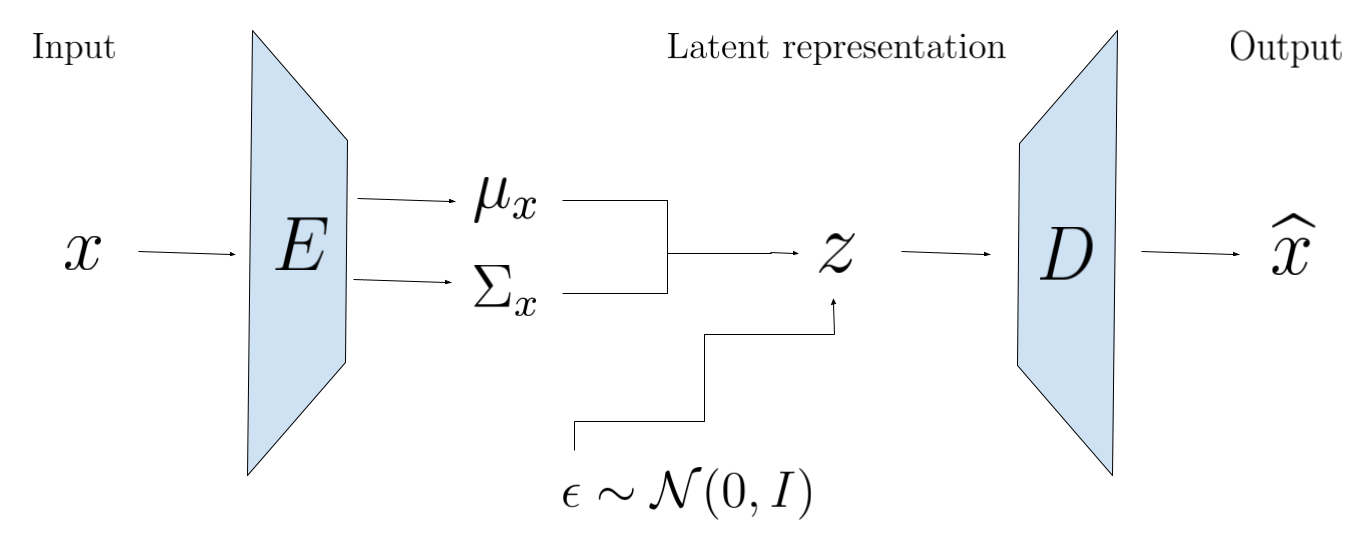
\includegraphics[scale = 0.2]{VAE_Normal.png}
    \centering
    \caption{Schematics of the VAE architecture with Gaussian reparameterization.}
    \label{fig:VAE_Normal}
\end{figure}


\subsubsection{Training objective}

As with other variational methods VAEs are optimized with respect to the \textit{evidence lower bound} or ELBO for short. Let $\x$ and $\z$ be two jointly distributed variables, with distribution $p_\theta$. Then for any distribution $q_\phi$ the ELBO is defined as

\begin{equation}
    \label{eq:ELBO}
    \loss_{\theta,\phi}(x) 
    = \mathbb{E}_{q_\phi(z|x)} \log \left( \frac{p_\theta(x,z)}{q_\phi(z|x)}\right)
\end{equation}
The ELBO can be reformulated in terms of the marginal likelihood and KL divergence of the variational to the true posterior.
\begin{equation}
    \begin{aligned}
        \label{eq:ELBO_loglik}
        \loss_{\theta,\phi}(x) 
        &=  \mathbb{E}_{q_\phi(z|x)} \log \left( p_\theta(x)\right) + \mathbb{E}_{q_\phi(z|x)} \log \left( \frac{p_\theta(z|x)}{q_\phi(z|x)}\right) \\
        &= \log \left( p_\theta(x)\right) - \textrm{KL}(q_\phi(z|x)|| p_\theta(z|x)).
    \end{aligned}
\end{equation}
Due to the non-negativity of the KL-divergence, we see that the ELBO bounds the marginal log likelihood of the data from below. By maximizing the ELBO with respect to the model parameters $\phi$ and $\theta$ one simultaneously maximizes the marginal likelihood, which improves the generative model, as well as reducing the KL-divergence of the approximate to the true posterior, which improves the inference model \cite{VAE}.\newline
An alternative reformulation gives a more evident connection to Autoencoders, with a the prior acting as a regularizer on the posterior 
\begin{equation}
    \begin{aligned}
        \label{eq:ELBO_AE}
        \loss_{\theta,\phi}(x) 
        &=  \mathbb{E}_{q_\phi(z|x)} \log \left( p_\theta(x|z)\right) - \mathbb{E}_{q_\phi(z|x)} \log \left( \frac{q_\theta(z|x)}{p_\phi(z)}\right) \\
        &= \underbrace{\mathbb{E}_{q_\phi(z|x)} \log \left( p_\theta(x|z)\right)}_{\text{Expected reconstruction log likelihood}} - \underbrace{\textrm{KL}(q_\phi(z|x)|| p_\theta(z))}_{\text{Regularizer}}.
    \end{aligned}
\end{equation}
As the $p_\theta(x|z)$ is typically assumed to be Gaussian we have

\begin{equation}
    \log p_\theta(x|z) = -\frac12 \left[k\log(2\pi)+ (x-D(z))^T(x-D(z))\right],
\end{equation}
which is equivalent, as an optimization objective of $D(z)$, to $||x-D(z)||_2^2$. Consequently the likelihood in the loss is implemented as the MSE of the input $x$ and the output $D(z)$.

\subsubsection{Generative model}
The role of the prior in a VAE is two fold. Firstly as a regularizing constraint for the posterior during training, and secondly as a way of obtaining new samples $x$ via ancestral sampling. Ancestral sampling refers to $\z$ being the parent node of $\x$ in the VAE, and that we can generate samples $x$ by drawing a sample $z\sim p(z)$ and decode $D(z)$. 




\TODO{Speak on limitations of VAE before introducing VQVAE}
Variational autoencoders has the issue of collapsing. Variance issues.


\subsection{Vector Quantization (VQ)}
Dictionary learning model \cite{Gray1984VQ}

\subsection{VQVAE}
The Vector Quantized Variational AutoEncoder (VQVAE) was first introduced in \cite{VQVAE} and presented a new way of training VAEs with discrete latent variables. It is the first discrete VAE model which has similar performance to the continuous variant. VQVAE was developed to learn useful discrete representations for generation. This is enforced by more flexible distributional assumptions, as they say "Our model, the Vector Quantised-
Variational AutoEncoder (VQ-VAE), differs from VAEs in two key ways: the
encoder network outputs discrete, rather than continuous, codes; and the prior
is learnt rather than static."-\cite{VQVAE}. 
\newline
The overall architecture of VQVAE consists of an encoder and decoder as before, together with a \textit{codebook} which is used in the quantization process. The codebook, also referred to as the latent embedding space, $\mathcal{Z} = \{z_k\}_{i=1}^K$ is consists of $K$ latent vectors with dimensionality $D$. It can be considered a lookup table of vectors that are used for vector quantization (VQ). The output of the encoder $E(x)$ is quantized by the means of nearest neighbor lookup
\begin{equation}
    z_q = \argmin_{z_k\in\mathcal{Z}} ||E(x)-z_k||.
\end{equation}

\begin{figure}[h]
    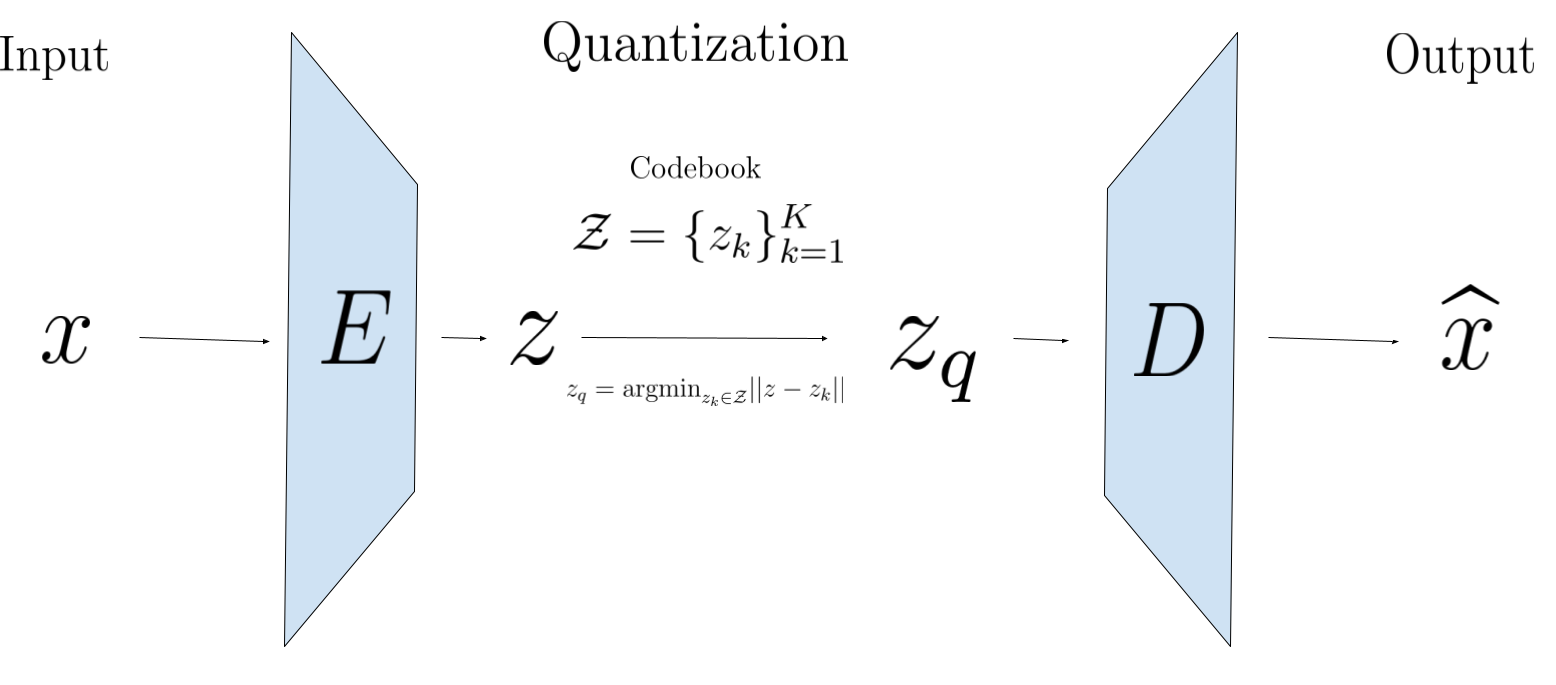
\includegraphics[scale = 0.2]{VQVAE.png}
    \centering
    \caption{Schematics of the VQVAE architecture.}
    \label{fig:VQVAE}
\end{figure}
From \ref{fig:VQVAE} we can see that the VQVAE can be seen as an autoencoder with a nonlinearity introduced by the vector quantization. \newline

In the original article \cite{VQVAE} they propose to separately learn the prior distribution, after the encoder, decoder and codebook is learned. During the initial training the prior is assumed to be uniform, which poses no constraint on the posterior learning. \newline

In contrast to VAEs the posterior is assumed to be categorical, as opposed to normal and the probabilities are defined as
\begin{equation}
    p(z=k | x) = 
    \begin{cases} 
        1 \quad \text{for }k = \argmin_j||E(x) - z_j||_2 \\
        0 \quad \text{otherwise}
    \end{cases},
\end{equation}
Sampling from the posterior amounts to quantizing the output of the encoder, as it is deterministic. \newline

VQVAE can be viewed as a VAE, hence we can bound the marginal likelihood with the ELBO \ref{eq:ELBO_AE}. As the variational posterior is deterministic and the prior (during training) is uniform over $\{1,...,K\}$ we get that the regularizing term

\begin{equation}
    \begin{aligned}
        \KL(q(z|x)||p(z)) &= \sum_{z}  q(z|x) \log \left(\frac{q(z|x)}{p(z)}\right) \\
                           &= q(z=k|x) \log \left(\frac{q(z=k|x)}{p(z=k)}\right) \text{, $q$ is deterministic}\\
                           &= \log \left(\frac{1}{1/K}\right) \text{, uniform prior}\\
                           &= \log(K), 
    \end{aligned}
\end{equation}
is constant. Consequently the ELBO reduces to the reconstruction term only. \newline

% \TODO{What do we gain by having a flexible posterior and a non-informative prior during training? The advantages for generative modelling to have a learnable prior? VAEs are traditionally quite bad when it comes to generative quality (sharpness). The flexibility of VQVAE seems to set the stage for better sample generation.}

\TODO{Can think of the codes as the modes of a mixture of Gaussians, and instead of sampling from the mixtrure you just choose the closest mode.}

\subsubsection{Prior Learning}
During the initial training the prior is as mentioned constant and uniform such that the posterior has more flexibility. After training an autoregressive prior is fit on $z$ so we can sample $x$ via ancestral sampling. The prior is learned with a generative objective, which increases the quality of generated samples. The choice of prior model depends on the particular application. In the original article PixelCNN \cite{oord2016pixel} was used for image, while WaveNet \cite{oord2016wavenet} was used for audio. More recently in TimeVQVAE \cite{TimeVQVAE} utilized a bidirectional transformer \cite{chang2022maskgit} for prior learning in the time series domain. 

\subsubsection{Loss funciton}
\label{section:VQVAELoss}
As we want to do gradient based learning, and the quantization process is quite far off from being continuous, measures has to be taken. The output of the encoder and the input of the decoder has the same dimension, which opens the possibility of simply copying the gradients from the decoder input to the decoder output. This is referred to as the \textit{straight through estimator}. The gradients from the decoder contains relevant information to how the encoder should change its output, and in the subsequent forward pass the encoder output can be quantized to different discrete latent codes.\newline

The loss function consists of two parts, the reconstruction loss, codebook loss. We already mentioned that the ELBO objective reduced to the reconstruction term only. In order to learn the codebook one uses the codebook loss, which is the euclidean distance between the encoder output and the quantized output, together with commitment term, which is introduced to keep the distance between codewords from growing arbitrarily large. To summarize the total loss is given by

    \begin{equation}     
        \label{eq:VQVAELoss}
        \begin{aligned}
            \loss_{\text{recons}} &= ||x - \widehat{x}||_2^2\\
            \loss_{\text{codebook}} &= ||sg(z) - z_q||_2^2 +\beta||z - sg(z_q)||_2^2\\
            \loss_{\text{VQ}} &= \loss_{\text{codebook}} + \loss_{\text{recons}}
        \end{aligned}
    \end{equation}

where $\beta$ is a tuning parameter typically set to be $0.25$ and $sg()$ is the stopgradient operation, defined to be the identity with zero partial derivatives. \newline

The VQ loss only affects the codebook, and can hence alternatively be updated as a function of moving averages of the encoder outputs $z$. This is expanded on in appendix A.1 in \cite{VQVAE}.\newline 

To illustrate the need for commitment term and what it does consider a model where the data is either $0$ or $1$ and we initialize the codebook with $\mathcal{Z} = \{-1,1\}$.  The range of the encoder is $\R$ and $E(x)$ is quantized to $-1$ if its negative and $1$ if its positive. Assume that the encoder and decoder will try to differentiate between the two classes by pushing $E(0)$ and $E(1)$ away from each other. As the reconstruction loss only affects the encoder and decoder, and the codebook loss only affect the codebook, we get that when the encoder and decoder parameter trains faster than the codebook, then the distance between the encodings and the codewords will steadily increase and the codebook loss diverge. This behavior is observed experimentally. \newline 


\section{Evaluation metrics}

\subsection{Tokenization model}

The tokenization model, as we are interested in representation learning, is evaluated on two metrics. Firstly, and most importantly its ability to reconstruct the input data once compressed into latent space. In essence the latent representation encodes "everything" (important information is preserved) about the original data if the model is able to reconstruct well. Secondly we evaluate linear classifiers on the latent representations, which provides good results if the model learns discriminative features of the different classes and produces an approximately linear separable space. Finally, as the tokenization model is a part of the generative model, the ultimate evaluation metric is the corresponding evaluation of the generative model. 

\subsubsection{Reconstruction}


\subsubsection{Downstream Classification}

SVM, KNN. The difference in inductive bias for the two classifiers. 


\begin{figure}[h]
    \label{fig:ClassifierComparrison}
    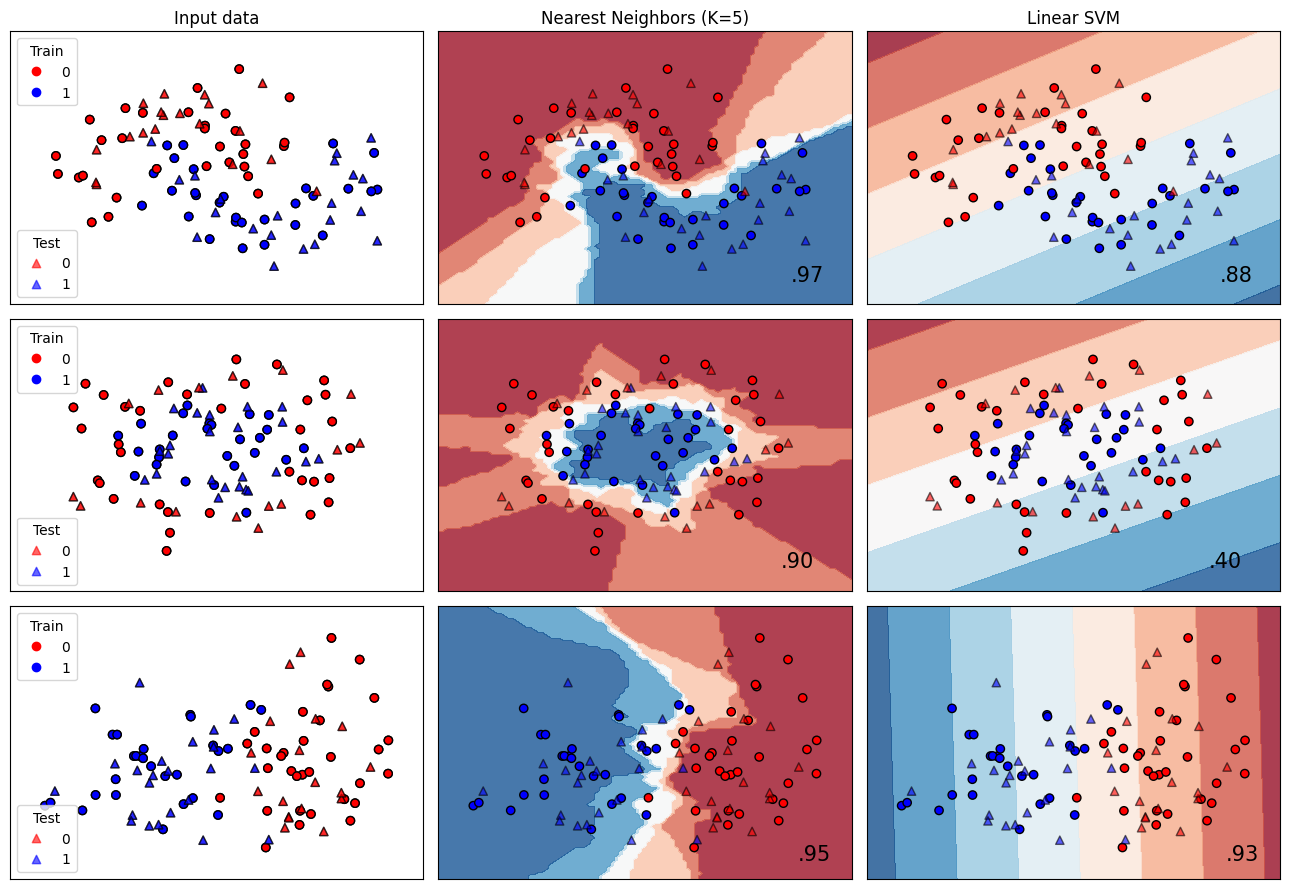
\includegraphics[scale = 0.4]{ClassifierComparrison.png}
    \centering
    \caption{Modified example taken from \url{https://scikit-learn.org/stable/auto_examples/classification/plot_classifier_comparison.html}.}
\end{figure}

\subsection{Generative model}
Good evaluation protocols for generative models are hard to come by, and the hunt for such is an active area of research. There are data modalities for which such evaluation metrics have more established standards than others. Most notably in the computer vision domain there is a benchmark dataset (ImageNet) and classifier (Inception v3). \newline

The typical sanity check for generative models is human visual inspection. In development of evaluation metrics for generative models, how well a proposed metric correlates with quality determined by visual inspection is standard. Most people know what cats and dogs look like and can recognize features even in crudely generated images. In contrast, many time series dataset measure quantities and signals for which the untrained eye has no idea of determining the quality. This is one of the obstacles in TSG. Despite this, according to \cite{TimeVQVAE} the most common evaluation protocols in the TSG literature is PCA and t-SNE analyses on time series to visually see similarities of two distributions. The major limitations of this is that the visual inspections cannot be reduced to a single score, which makes objective comparison difficult. \newline

Following \cite{TimeVQVAE} we mainly consider three evaluation metrics in this thesis. \textit{Inception Score} (IS), \textit{Fréchet Inception Distance} (FID) and \textit{Classification Accuracy Score} (CAS). IS measures quality of synthetic samples using the entropy of the label distribution and the evenness in prediction across labels. The \textit{Fréchet Inception Distance} measures a distance between the generative and ground truth distribution. Finally the \textit{Classification Accuracy Score} measures the quality of the class-conditionally generated samples by training a classifier on synthetic data and testing on real.

Common for all the above evaluation metrics is the reliance on a pre-trained classification model. In contrast to computer vision there is no widely adopted classification model for time series, but in \cite{wang2016time} a fully convolutional network (FCN) was presented as a proposed baseline classification model for time series. As their model is not available we use the open source FCN trained on the UCR Archive presented in \cite{TimeVQVAE} for our evaluations.\newline

\subsubsection{Inception Score (IS)}
Inception Score (IS) was first introduced in \cite{salimans2016improved} as an automatic evaluation method of synthetic samples.\newline
The Inception Score works by applying a classifier to every generated sample to get the conditional label distribution $p(y|x)$. Samples containing clear characteristics should have low entropy, i.e one should be certain of the label. In addition we expect a good model to generate varied samples, so the marginal $\int p(y|x = D(z))dz$ should have high entropy. On this basis, the Inception Score is defined as 

\begin{equation}
    \label{IS}
    {\text{IS}}(\theta) = \exp\left( \mathbb{E}(D_{\text{KL}}(p_\theta(y|\mathbf{x}) || p_\theta(y))) \right).
\end{equation}

In contrast to computer vision there is no widely adopted classification model for Time Series. In \cite{wang2016time} a fully convolutional network (FCN) was presented as a proposed baseline classification model, and we use the open source FCN trained on the UCR Archive presented in \cite{TimeVQVAE} for our evaluations. \newline

Let $X_{\text{gen}} = \{x_{i,\text{gen}}\}_{i=1}^N$ be a set of generated samples. We use the apply a SoftMax layer to pretrained FCN representations to obtain an estimate of the conditional label distribution as follows
\[
    x_{i,\text{gen}} \xrightarrow{\mathrm{FCN} + \mathrm{SoftMax}} p(y |x_{i,\text{gen}}).
\]
The marginal label distribution is obtained by averaging across all the synthetic data as follows

\[
    p(y) = \frac{1}{N} \sum_{i=1}^N p(y |x_{i,\text{gen}}).
\]

Issues with IS \cite{barratt2018note} (Use different network, for image classification).  Important to report different metrics that indicate that the model has not overfitted. 
Also issues with IS \cite{borji2021pros}.\newline

\subsubsection{Fréchet Inception Distance (FID)}
As an attempt to improve on IS \cite{heusel2018gans} introduced the Fréchet Inception Distance (FID). Since then FID has been the standard for assessing generative models \cite{borji2021pros}.\newline
The primary concern with IS is, as mentioned earlier, that it does not use any statistics of real world samples to compare with the statistics of the generated samples. In contrast FID relates the synthetic sample to the real world samle via the \textit{Fréchet distance}. For any two probability distributions, $f,g$ over $\R^n$, with finite mean and variances, their  distance is defined as 
\begin{equation}
    \begin{aligned}
        d_F(f,g) &= \left(\inf_{\gamma \in \Gamma(f,g)} \int_{\R^n\times\R^n}||x-y||_2^2d\gamma(x,y) \right)^{\frac{1}{2}}\\\\
            &= \left(\inf_{\gamma \in \Gamma(f,g)} \E_{(x,y)\sim \gamma} ||x-y||_2^2\right)^{\frac{1}{2}},
    \end{aligned}
\end{equation}
where $\Gamma(f,g)$ is the set of all \textit{couplings} of $f$ and $g$. The Fréchet distance is a special case of the Wasserstein metric and will in literature be referred to as such.\newline 

In \cite{DOWSON1982450} it was shown that for two Gaussian distributions the Fréchet distance is explicitly solvable as

\begin{equation}
    \label{eq:FID Gaussian}
    d(\N(\mu,\Sigma),\N(\mu',\Sigma'))^2 = ||\mu-\mu'||_2^2 + \Tr \left( \Sigma + \Sigma' - 2(\Sigma\Sigma')^{\frac12}\right)
\end{equation}

The \textit{Fréchet Inception Distance} is an application of the Fréchet distance on the representation distributions from a specified model. The models are Inception v3 in the image domain and SupervisedFCN in the time series domain.\newline

In \cite{heusel2018gans} they argue that since the Gaussian distribution is the maximum entropy distribution over $\R^n$ for a given mean and covariance it is a reasonable distribution to assume for the representations. The mean and covariance is estimated from the samples and the explicit formula \ref{FID Gaussian} is used to calculate the FID. \newline

FID is not without fault, and the Gaussian assumption has been shown not to hold \cite{jayasumana2024rethinking}. Further, as the FID relies on estimating large covariance matrices, a large number of samples is needed to obtain a reliable estimate.\newline

Rethinking FID: \cite{jayasumana2024rethinking} \newline

\cite{chong2020effectively} FID and IS are biased.\newline

FID score measures difference in the distribution of representations of time series. The representations capture high level semantics of the time series and analyses of these representations can provide greater insights to the realism of generated samples. \newline


\subsubsection{Classification Accuracy Score (CAS)}
% \cite{smith2020conditional} report the CAS.
A method for evaluating the models ability to learn class conditional distributions is to train a separate classifier on the on synthetic data and test on real data (TSTR). That is we generate $N$ synthetic samples $\{x_i,y_i\}_{i=1}^N$ using class conditional sampling. We then train a classifier on this synthetic dataset, and evaluate the CAS of this classifier on a real test dataset. High CAS values indicate that the generative model produces samples similar to the real data and captures relevant class specific features.\newline

We evaluate the CAS for TSTR by using the Supervised FCN introduced in \cite{TimeVQVAE} on all our models considered and compare against the baseline model to investigate the relative performance. 



\end{document}